%%==================================================
%% chapter01.tex for BIT Master Thesis
%% modified by yang yating
%% version: 0.1
%% last update: Dec 25th, 2016
%%==================================================
\chapter{国内外研究工作概述}
\label{chap:recent_work}
本章分别介绍事件检测和两种不同定义下的事件要素抽取技术的发展脉络,并梳理各自存在的共有问题,分析研究思路。

\section{事件检测}
事件检测(Event Detection)是从文本中抽取结构性事件知识的关键步骤~\cite{grishman1997information,ahn2006stages},其旨在识别出具有特定事件类型的事件触发词。事件检测是以事件为中心的信息抽取技术的必要基础,在建模事件要素抽取、事件关系抽取和事件事实性识别等事件知识图谱构建任务时不可或缺,同时也
广泛应用于社交内容分析~\cite{zhou2017event}、知识系统~\cite{li2020gaia,wen2021resin}、故事生成~\cite{li2022event}等多种任务中。

早期的事件检测主要基于模式和特征进行建模。其中,基于模式的方法先构造事件模式,然后在抽取阶段根据事件模式匹配出对应的事件检测信息。事件模式一般基于原始文本或注释信息构建,在早期发展阶段由具备专业语言学知识的专家进行创建。进一步,一些研究利用少量事件模式种子,结合弱监督方法或自助法(Bootstrapping)实现更多事件模式的自动获取~\cite{xu2006automatic,liao2010filtered,kilicoglu2011effective,cao2015improving2}。

而基于特征的方法研究将事件检测分类的线索特征转化为特征向量,并使用机器学习方法进行建模。这些特征可以被划分为局部特征和全局特征。局部特征主要为词法特征和句法特征,包括完整的词、词性标签和依存句法特征等。例如,Chieu等人~\cite{chieu2002maximum}引入一元文法和二元文法等特征信息,并利用最大熵分类器(Maximum Entropy
Classifier)进行事件的检测。Chen等人~\cite{chen2009language}将包括前续字符、现有字符和后续字符的字符级别特征与词级别特征进行结合,并基于最大熵马尔可夫模型(Maximum Entropy Markov Model)检测中文事件触发词。而全局特征则不限于从事件触发词所在句子中得到,其可以为基于跨句子、跨文档和跨事件等获取的实体类型、事件要素信息和词义信息等~\cite{ji2008refining,gupta2009predicting,liao2011acquiring,hong2011using,li2013joint,li2015improving},通常被用于局部信息的补充。例如,Ji等人~\cite{ji2008refining}将相关文档中相同词在不同事件实例中的语义一致性作为全局信息依据,辅助局部的事件预测。Liao等人~\cite{liao2011acquiring}构建无监督主题模型如LDA(Latent Dirichlet Allocation),以获取文档级别的全局信息,用于事件检测任务。Li等人~\cite{li2013joint}在建模中融合了不同事件的依赖关系,如事件触发词间的依赖路径和上下文信息。然而,基于特征的方法通常使用独热向量表示构造的特征,易导致数据稀疏问题。更重要的是,不管基于模版还是特征的方法,都需要具备语言学知识的专业人士进行构建,对于一些低资源语言来说人力成本变得更加昂贵。因此,随着深度学习技术的快速进步,其能够自动从文本中学习语义表示的优势在事件检测任务中得以突显。接下来,本章根据使用的神经网络架构类型进行分别介绍。

\subsection{基于卷积神经网络的方法}

卷积神经网络(Convolutional Neural Networks,CNN)实质为多层感知机的变种形式,受益于其卷积核带来的权重共享和较小感受野,能够以较小的参数规模和计算复杂度实现特征信息的获取。在自然语言处理中,通常将传统二维卷积核的其中一个维度设置为词向量的维度,只改变另一维卷积操作的尺寸大小,将文本中多个词(或字符)组成的片段信息线性映射到特征空间中~\cite{zhang2015sensitivity},实现自动捕捉这些文段的语义和句法信息。具体来说,给定$n$个词组成的句子文本$\left\{w_{1}, w_{2}, \cdots, w_{n}\right\}$,对应的向量输入为$\left\{\boldsymbol{x}_{1}, \boldsymbol{x}_{2}, \cdots, \boldsymbol{x}_{n}\right\}$,假设卷积窗口大小为$k$,则可得任意一个利用该卷积核运算的特征结果:
\begin{equation}
    a_{i}=f\left(\boldsymbol{W} \otimes \boldsymbol{x}_{i: i+k-1}+b\right)
\end{equation}
其中$\boldsymbol{W}$和$b$为待学习训练的参数,$f(\cdot)$为激活函数,$\boldsymbol{x}_{i: i+k-1}$表示从向量$\boldsymbol{x}_{i}$到$\boldsymbol{x}_{i+k-1}$的拼接,$\otimes$为卷积计算。在实际应用中,为了建模特征的多样性,在每个卷积层中采用多个卷积核进行对应特征的捕捉。

在事件检测中,Nguyen和Grishman~\cite{nguyen2015event}为最早应用CNN的研究者。在其构建的方法中,首先将文本中每个词对应的词向量、实体类型向量和相对于目标预测词的位置向量进行串接,然后输入到包含不同尺寸卷积窗口的卷积层中,最后通过最大池化操作得到目标词的特征表示,从而进行最终的事件预测。为了在编码词法特征和句法特征时能够更多地关注到事件触发词信息,Chen等人~\cite{chen2015event}在DMCNN模型中提出了一个动态池化操作去替代传统的最大池化操作,其根据目标预测词的位置将经过卷积层得到的特征表示划分为两部分,分别进行最大池化操作。如图\ref{dmcnn}所示,根据“died”的位置将卷积层得到的向量表示划分为两个部分进行池化处理。与使用卷积层挖掘连续文段信息不同,Nguyen等人~\cite{nguyen2016modeling}设定窗口长度并枚举所有符合该长度要求的非连续文段。然后,使用卷积层建模这些文段,并采用动态规划算法得到其中语义信息最显著的序列,用于最终的事件预测,从而实现非连续词间的长依赖信息的获取。

\begin{figure}[htp]
   \centering
   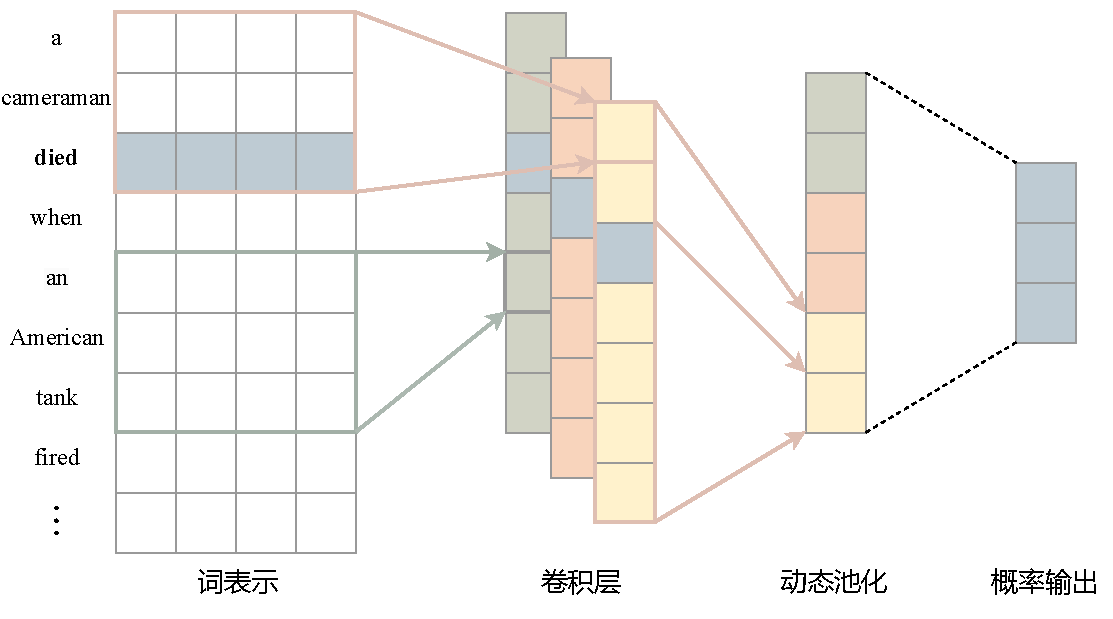
\includegraphics[width=0.8\linewidth]{figures/chap2/dmcnn.pdf}
   \caption{DMCNN模型示意图}
   \label{dmcnn}
\end{figure}

\subsection{基于循环神经网络的方法}

循环神经网络(Recurrent Neural Networks,RNN)\cite{rumelhart1986learning}常用于序列信息的建模,其与传统的全连接网络不同,每层的节点之间存在连接,从而能够更好地捕捉序列中的顺序关联。由于自然语言文本可以视作词组成的序列,RNN可以高效利用到单词顺序对特征编码和结果预测的影响,因而广泛应用在自然语言理解和自然语言生成任务中。具体地,如图\ref{rnn}所示,传统的单步RNN可以看作是相同的计算操作在不同时间步的重复叠加组合,假设$n$个词组成的文本序列向量输入为$\left\{\boldsymbol{x}_{1}, \boldsymbol{x}_{2}, \cdots, \boldsymbol{x}_{n}\right\}$,则第$t$个时间步对应的输出向量$\boldsymbol{y}_{t}$可得:
\begin{equation}
    \begin{aligned}
& \boldsymbol{h}_t=f\left(\boldsymbol{W}^h\left(\boldsymbol{h}_{t-1} ; \boldsymbol{x}_t\right)+\boldsymbol{b}^h\right) \\
& \boldsymbol{y}_t=g\left(\boldsymbol{W}^y \boldsymbol{h}_t+\boldsymbol{b}^y\right)
\end{aligned}
\end{equation}
其中$f(\cdot)$和$g(\cdot)$通常为非线性激活函数,$\boldsymbol{h}_t$为当前时间步的隐藏层状态向量,$\boldsymbol{W}^h$、$\boldsymbol{W}^y$、$\boldsymbol{b}^h$和$\boldsymbol{b}^y$为不同时间步共享的训练参数。进一步,以LSTM~\cite{hochreiter1997long}和GRU~\cite{cho2014learning}为代表的RNN变体被提出,以缓解传统RNN建模长序列时产生的梯度消失和梯度爆炸现象。

\begin{figure}[htp]
   \centering
   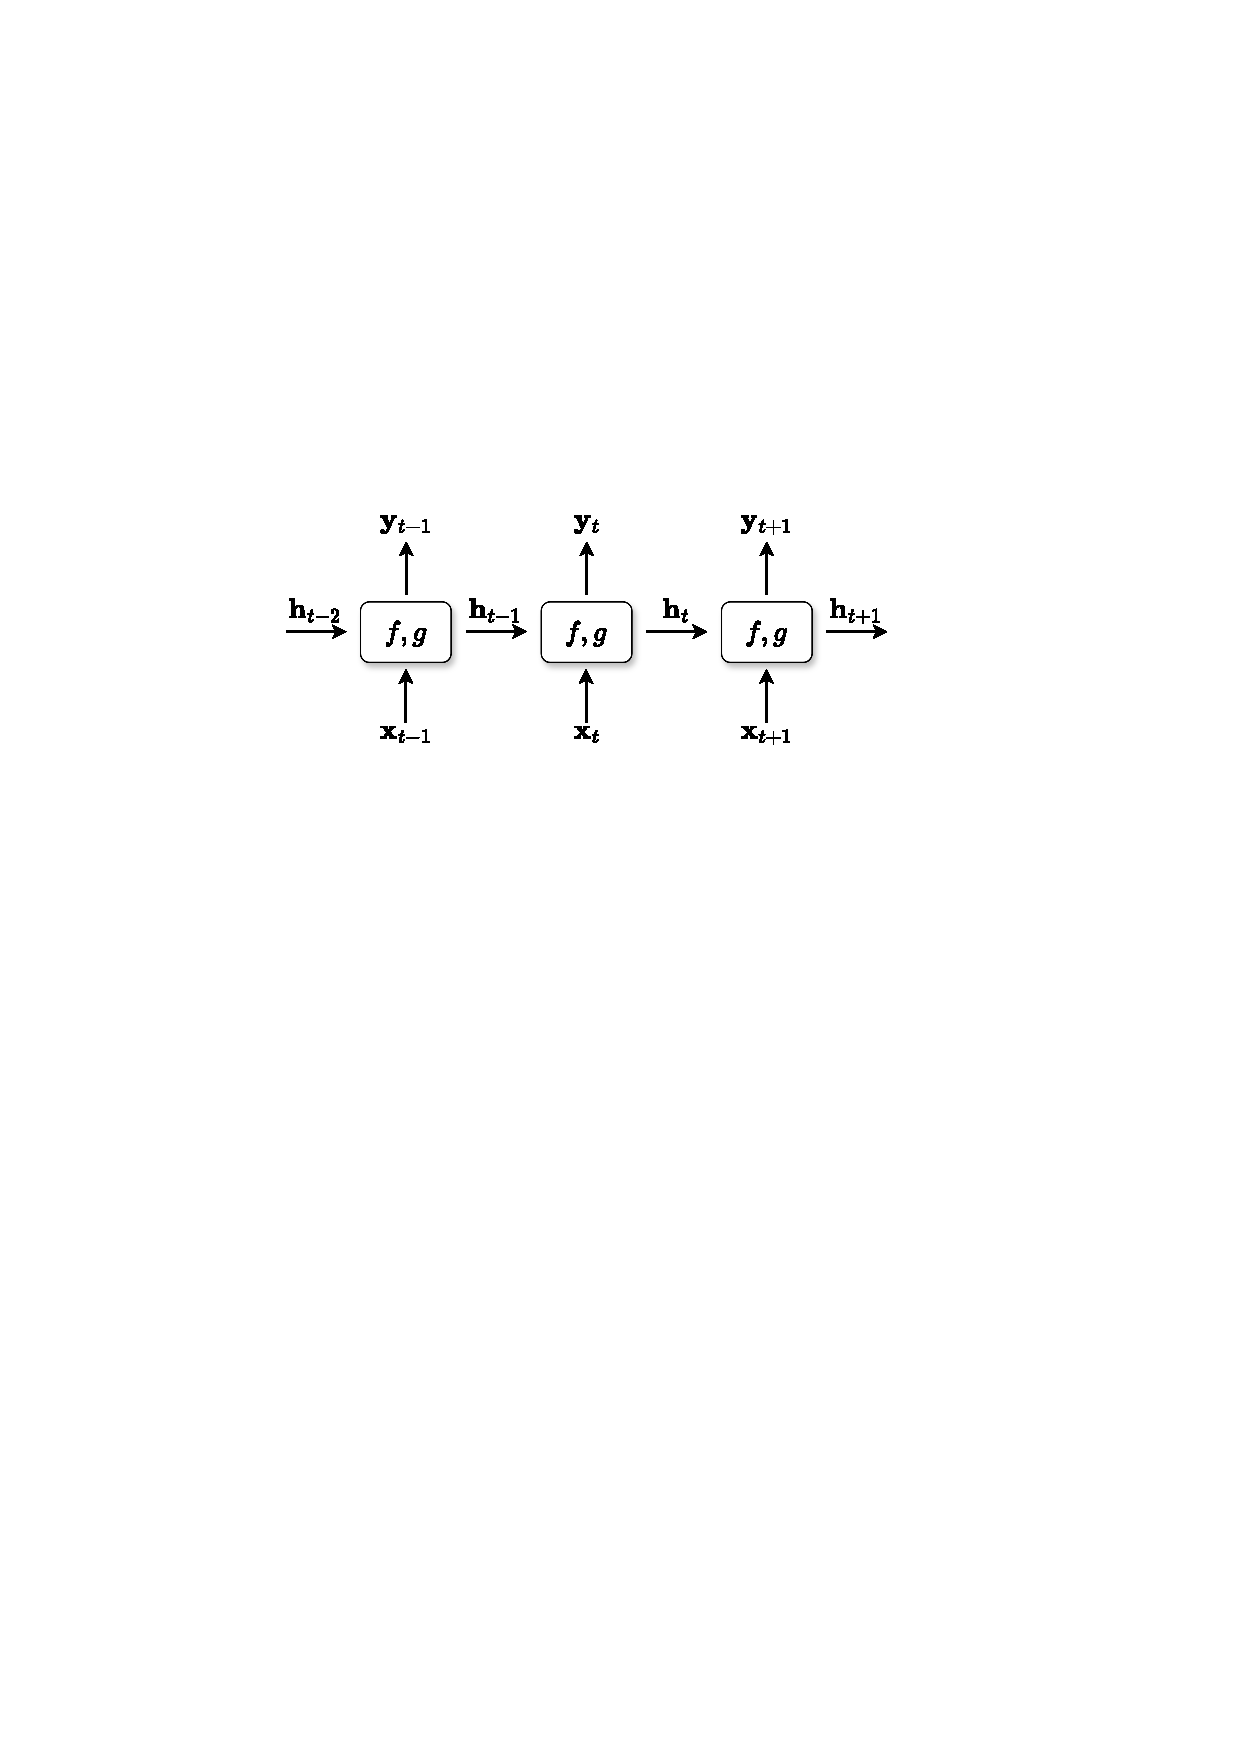
\includegraphics[width=0.7\linewidth]{figures/chap2/rnn.pdf}
   \caption{RNN示意图}
   \label{rnn}
\end{figure}

在事件检测任务中,Ghaeini等人~\cite{ghaeini2016event}最先应用了LSTM,其根据候选触发词将文本划分为左侧上下文、候选触发词本身和右侧上下文,分别使用LSTM进行编码并进行特征表示的串接,以用于最终的多分类事件预测。Jagannatha等人~\cite{jagannatha2016bidirectional}则将医疗领域的事件检测转化为序列标注问题,结合预定义事件类型和BIO(Begin,Inside,Outside)标注策略,使用双向LSTM或GRU进行建模。Orr等人~\cite{orr2018event}将依存句法信息转化为有向非循环图,并基于GRU提出了一个新的变种模型,以更好地在事件检测中利用句法信息和上下文信息。为了解决GRU和LSTM等网络中门控计算依赖之前时间步的信息而导致的无法并行计算的问题,Zhang等人~\cite{zhang2019empower}基于简单循环单元(Simple Recurrent Unit,SRU),构建两个SRU模型分别用于获取事件检测中单词级别和字符级别的语义特征,以实现性能和计算效率的更好平衡。

虽然RNN相比于CNN能够建模更长的词间依赖关系,但其建模的有效上下文长度仍然受限,为了进一步提高上下文信息的利用效率,一些研究者在此基础上引入了注意力机制。例如,Chen等人~\cite{chen2018collective}利用跨句信息和不同事件间的相关性增益事件检测的性能。在该模型中,其一方面基于双向LSTM网络在句子级别得到每个词的特征表示,然后使用两层注意力机制获取对应的文档级别特征表示,并构建门控机制实现不同级别信息的融合。另一方面,其构建了多层LSTM的变体网络层TLSTM,其在LSTM门控计算中增加了通过注意力机制得到的前一层预测的所有词的事件类型标签信息,从而隐式地构建不同事件预测结果的关联性。Lou等人~\cite{lou2021mlbinet}同样基于LSTM网络和注意力机制构建一个编码器-解码器架构,以利用跨句范围内的语义信息和事件间的依赖关系。在编码器中,使用双向LSTM网络进行编码,并基于自注意机制融合长距离上下文语义信息。在解码器中,分别使用融合了前一个词标签预测信息的双向RNN解码器,并串接相应的解码表示,以获取能够双向捕捉同一句子内不同事件关联依赖的事件标签向量。进一步考虑到跨句范围的事件依赖关系,其引入了另一个LSTM网络编码已得到的事件标签向量,从而聚合跨句范围内不同句子的整体事件信息。最后,为了能够在解码中利用到聚合的事件信息,作者们再次叠加新的双向解码层并融合前后相邻句子的事件信息。通过重复该融合过程,更远距离的句子事件信息得以被捕获,从而增益目标事件的检测。Liu等人~\cite{liu2019event}探索不依赖事件触发词标注信息去预测文本中存在的事件。作者们将该预测过程建模为多标签问题,使用LSTM编码得到词的特征表示,并使用不同的预定义事件类型向量作为查询向量,得到相应的文本整体表示,以预测对应事件类型的存在。

此外,一些研究针对CNN和RNN的特点,探索融合各自的优势进行事件检测任务的建模。例如,Feng等人~\cite{feng2018language}提出了一个融合CNN和RNN的混合神经网络,以用于多语言场景下的事件检测任务。其在使用双向LSTM网络建模上下文序列信息的同时,利用CNN获取局部文本特征表示。然后,串接这两种建模网络得到的信息,以进行多种语言数据集中的触发词检测。Lu等人~\cite{lu2019distilling}认为现有事件检测模型具备良好地区分不同上下文中容易混淆的高频触发词的能力,但缺乏识别罕见或未出现的触发词的泛化知识。为此,其一方面结合了RNN和注意力机制,建模以候选触发词为中心的上下文表示,以提供事件检测的触发词区分能力,并构建额外的二分类辅助任务增强候选触发词对其上下文表示的影响。另一方面,使用DMCNN~\cite{chen2015event}建模与候选触发词无关的上下文表示,以提供事件检测的触发词泛化能力。并且,利用生成对抗技术~\cite{creswell2018generative}降低候选触发词对其上下文表示的影响。最后,基于门控机制实现不同上下文表示的高效融合,以增强事件检测的整体性能。

\subsection{基于图神经网络的方法}

句法表示能够提供单词与其句法相关上下文的直接连接,但无论CNN还是RNN,均主要聚焦于建模自然语言文本中的序列。因此,为了更加高效直接地利用这类句法信息,近年来基于图进行建模的图神经网络(Graph Neural Networks,GNN)在自然语言处理的各个领域均得到广泛应用。在事件检测任务中,主要使用的是GNN中的图卷积神经网络(Graph Convolutional Neural Networks,GCN)\cite{kipf2016semi}。给定图$\mathcal{G}=(\mathcal{V}, \mathcal{E})$,其中$\mathcal{V}$为图中节点的集合,$\mathcal{E}$为图中边的集合。假设第$l$层图卷积的特征表示$\boldsymbol{H}^l=\left\{\boldsymbol{h}_i^l\right\}$,则第$l+1$层图卷积的特征表示可计算如下:
\begin{equation}
    \boldsymbol{h}_i^{l+1}=f(\sum_{(i, j) \in \mathcal{E}} \alpha_{i j}^l \boldsymbol{W}^l \boldsymbol{h}_j^l+\boldsymbol{b}^l)
\end{equation}
其中$\boldsymbol{W}^l$和$\boldsymbol{b}^l$为待学习训练的参数,$f(\cdot)$为非线性激活函数,$\alpha_{i j}^l$为节点$i$指向节点$j$的边对应的权重值。图\ref{gcn}展示了由四个节点组成的一个GCN示例。

\begin{figure}[htp]
   \centering
   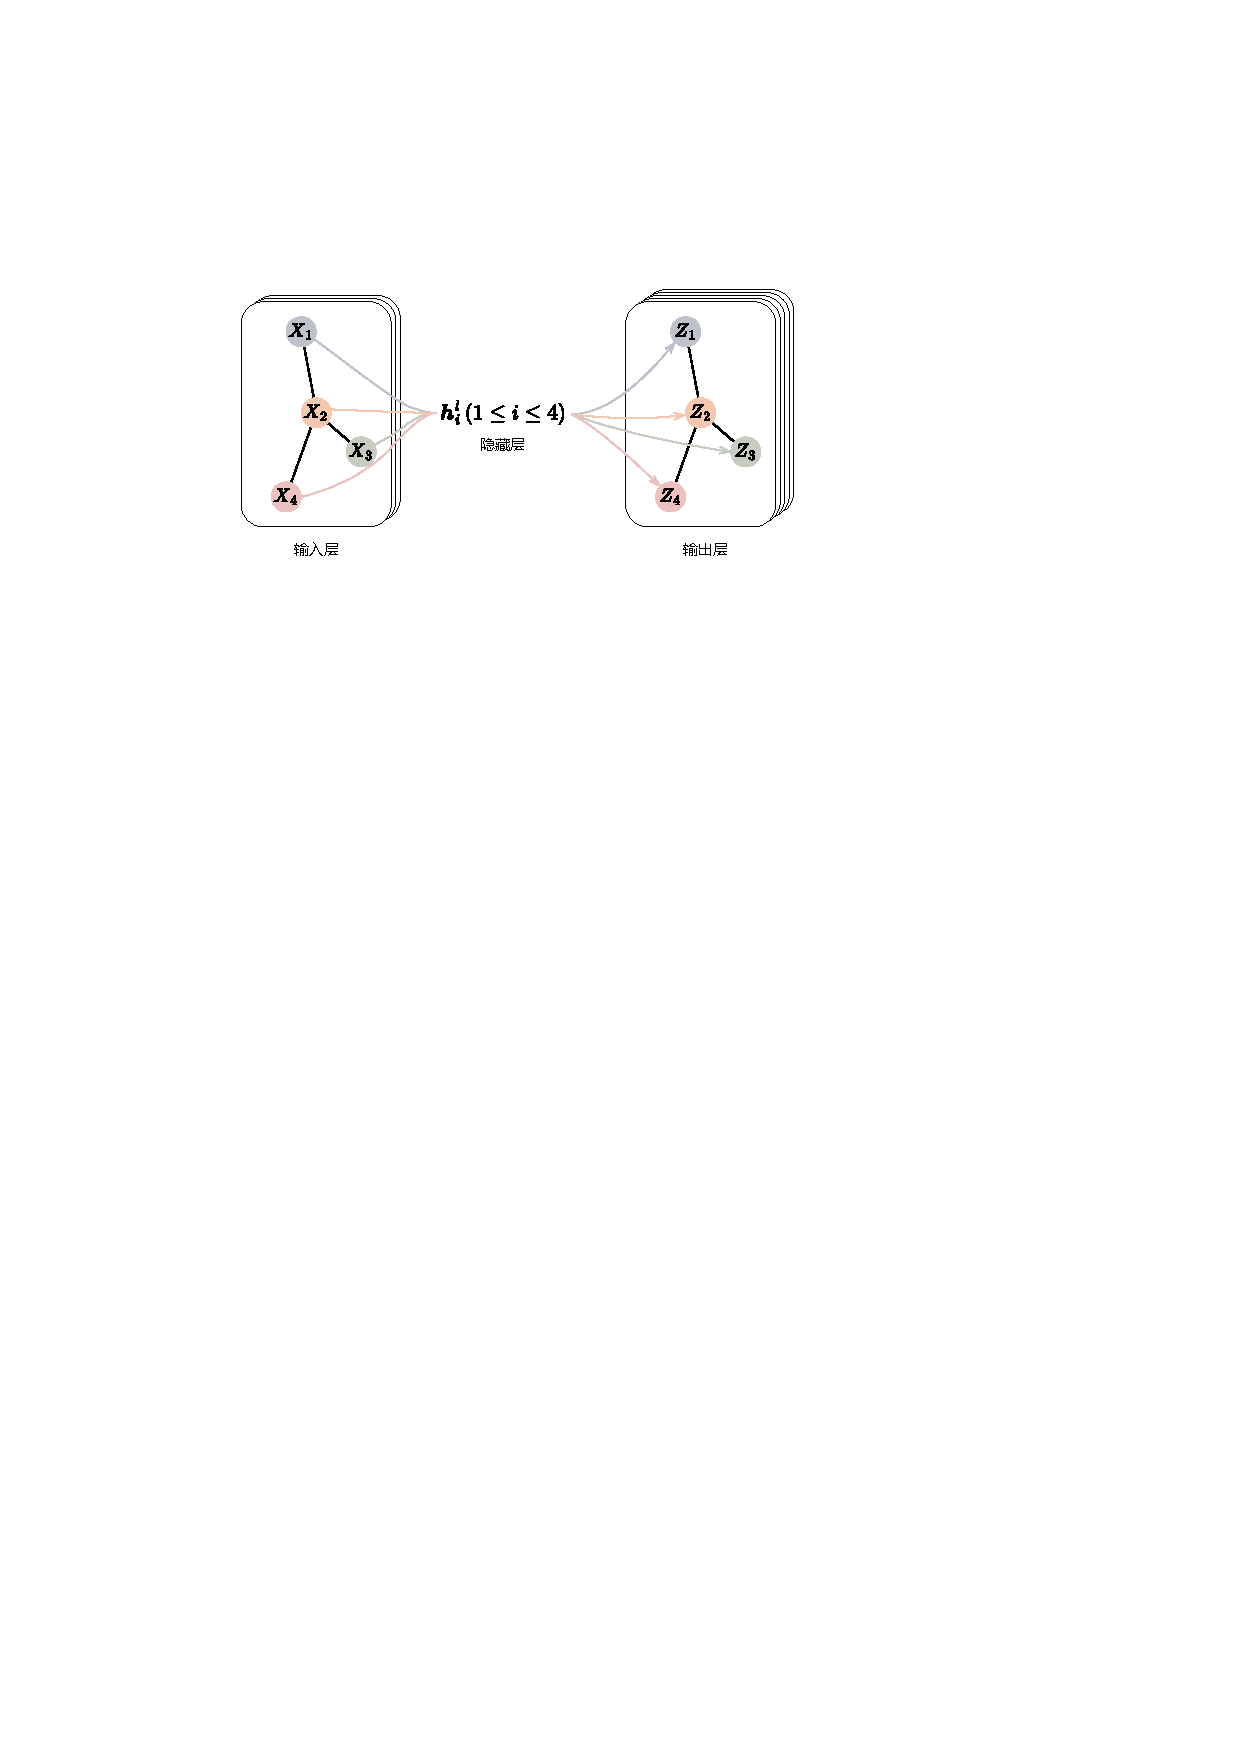
\includegraphics[width=0.7\linewidth]{figures/chap2/gcn.pdf}
   \caption{GCN示意图}
   \label{gcn}
\end{figure}

Liu等人~\cite{liu2018jointly}和Nguyen等人~\cite{nguyen2018graph}为最早在事件检测任务中使用GCN的研究者。在其研究工作中,首先使用自然语言处理工具将文本解析成结构化的依存句法树,然后设计策略将得到的依存句法树转化成可以用于建模GCN的图。具体地,图中的节点为句子中所有的单词,而节点间的边可以区分为三类。第一类边为直接从依存句法树中得到的正向边。假设在该树结构中,从单词$w_{i}$到单词$w_{j}$存在任意类型的依存句法关系,则在图中构建由节点$i$指向节点$j$的有向边。第二类边为所有第一类边的逆向边,以保证图中信息的逆向传播。第三类边则为每个节点指向自身的闭环边,使得构建的图能够形成闭环。基于所构建的图,进行多层GCN的迭代,实现依存句法树中多跳依存信息的高效获取。首先,利用双向LSTM网络层进行编码,以捕捉序列上下文信息。进一步,将编码得到的特征表示输入到GCN中,以获取构建的图中的结构化信息,其中不同类型的边使用不同的学习训练参数$\boldsymbol{W}^l$和$\boldsymbol{b}^l$,权重值$\alpha_{i j}^l$计算如下:
\begin{equation}
    \alpha_{i j}^l=\sigma(\boldsymbol{h}_j^l \boldsymbol{V}^l+d^l)
\end{equation}
其中$\boldsymbol{V}^l$和$d^l$为权重计算时学习的参数,且同一种类型的边计算时进行参数共享。$\sigma(\cdot)$为sigmoid激活函数。为了进一步在GCN中减少与候选触发词无关的信息干扰,Lai等人~\cite{lai2020event}基于候选触发词的特征表示生成对应的门控向量,从而实现对其他单词特征表示的过滤筛选:
\begin{equation}
    \boldsymbol{g}^l=\sigma\left(\boldsymbol{W}_g^l \boldsymbol{e}_t\right)
\end{equation}
\begin{equation}
    \boldsymbol{m}_i^l=\boldsymbol{g}^l \odot \boldsymbol{h}_i^l
\end{equation}
其中$\boldsymbol{W}_g^l$为学习的参数,$\boldsymbol{e}_t$为候选触发词在输入GCN前的编码表示,$\odot$为元素依次相乘操作。基于该门控方法获取的不同单词特征表示,最终用于辅助候选触发词的事件预测。此外,由于图网络中不同层建模上下文语义信息的侧重点有所不同,因此需要保证门控向量的多样性。为此,其设计了额外的正则化损失减少相同门控向量筛选过滤同一单词不同层特征表示后的相似程度。同时,作者们利用依存句法树中的依赖路径距离指导模型更好地感知不同单词对于候选触发词的重要程度。

此外,由于在事件检测常用的ACE2005数据集中,超过一半的事件触发词在其对应的依存句法树中和关联实体或者单词没有直接的连接。为此,Liu等人~\cite{liu2018jointly}和Nguyen等人~\cite{nguyen2018graph}通过叠加多层GCN进行建模。然而,随着GCN层数的叠加,图中节点的特征表示将会变得愈加相似,导致过平滑问题~\cite{zhou2020graph}。为了解决该问题,Yan等人~\cite{yan2019event}直接构建包含多跳依存句法关系的图,以替代在基于单跳依存句法关系构建的图上叠加多层GCN。与Liu等人~\cite{liu2018jointly}和Nguyen等人~\cite{nguyen2018graph}使用相同的策略,其首先将解析得到的依存句法树转化成包含正向边、逆向边和闭环边三种类型的有向图。不同的是,Yan等人~\cite{yan2019event}进一步根据各个类型得到对应的邻接矩阵,并计算任意$k$跳依存句法关系图的邻接矩阵如下:
\begin{equation}
    \boldsymbol{A}_{ type}^k=\left(\boldsymbol{A}_{type}\right)^k
\end{equation}
其中$\boldsymbol{A}_{type}$可为正向边、逆向边和闭环边分别对应的邻接矩阵。基于$\boldsymbol{A}_{ type}^k$,为了捕捉到依存句法树中单词间$k$跳的句法关系,其使用单层图注意力网络(Graph Attention Network,GAT)\cite{velivckovic2017graph}替代多层GCN进行编码如下:
\begin{equation}
    \boldsymbol{h}_i=f( \sum_{j=1}^n\left(u_{i j} a_{i j}\left(\boldsymbol{W}_{a} \boldsymbol{p}_j+\boldsymbol{\epsilon}\right)\right))
\end{equation}
\begin{equation}
    u_{i j}=\frac{\exp \left(e_{i j}\right)}{\sum_{j \in \mathcal{N}_i} \exp \left(e_{i j}\right)}
\end{equation}
其中$e_{i j}=g\left(\boldsymbol{W}_1\left[\boldsymbol{W}_2 \boldsymbol{p}_i;\boldsymbol{W}_2 \boldsymbol{p}_j\right]\right)$,$\boldsymbol{W}_1$、$\boldsymbol{W}_2$、$\boldsymbol{W}_{a}$和$\boldsymbol{\epsilon}$为待学习训练的参数,$a_{i j}$表示$\boldsymbol{A}_{ type}^k$对应的图中节点$i$指向节点$j$的边对应的权重值,$\boldsymbol{p}_j$为图中节点$j$的输入向量,$\mathcal{N}_i$表示在$\boldsymbol{A}_{ type}^k$对应的图中节点$i$的邻接节点集合,$f(\cdot)$和$g(\cdot)$分别表示ELU和LeakyReLU激活函数。最后,利用注意力机制聚合每个单词在不同跳句法关系图上建模获取的特征表示,以用于最终的事件类型预测。

与上述研究工作不同,最近的方法考虑进一步利用依存句法关系的类型信息。Cui等人~\cite{cui2020edge}提出了在GCN中构造一个邻接张量,以利用其中的向量表示图中任意两个节点的关系。若图中节点间的依存句法关系类型相同,则对应的向量初始化也相同。基于此,分别设计了图中节点表示和边表示的相互迭代更新方法,以实现高效建模邻接张量中的异质信息。Liu等人~\cite{liu2021self}在Cui等人~\cite{cui2020edge}研究工作的基础上,考虑了依存句法树中句法关系存在方向性的区别,初始化了两个非对称的邻接张量。然而,静态的邻接张量仍无法有效建模依存句法信息之外不同节点间潜在的依赖关联,为此其进一步构建了一个自注意力模块,以动态更新自注意力张量,并融入到节点表示和边表示的迭代计算中。

此外,Mi等人~\cite{mi2022event}利用依存句法树和语义角色标注构造双重关系图,在考虑句法结构的同时,引入互补的语义关系信息,以减少句法信息带来的噪音和冗余。具体地,在构建双重关系图时,保留在依存句法树中与候选触发词直接连接的单词和句法关系,将其他句法关系替换成表示与候选触发词的连接距离的虚拟关系。同时,根据语义角色标注结果引入语义关系的连接。基于构建的关系图,构建关系增强的GAT,其基于对应关系向量和上下文信息进行注意力机制的权重计算。

\subsection{基于预训练语言模型的方法}
近年来,预先基于大规模无标签文本数据进行训练,再根据具体下游任务微调的建模方式广泛应用在各种自然语言处理任务中。在事件检测任务中,通常使用以BERT (Bidirectional Encoder Representations from Transformers)\cite{kenton2019bert}为代表的双向语言模型作为进一步微调使用的预训练语言模型。BERT主要由多层Transformer~\cite{vaswani2017attention}编码器组成,其每一层的架构如图\ref{transformer}所示。该架构由$N$(一般设置为6)个相同的子网络层组成,每个子网络层主要包括多头注意力和前馈神经网络,并辅以加和连接和层归一化操作。在多头注意力(MultiHead)中,并行学习$h$组不同的线性变换层参数分别将自注意力计算输入中的键矩阵$\boldsymbol{K}$、值矩阵$\boldsymbol{V}$和查询矩阵$\boldsymbol{Q}$映射到各自的特征空间中,然后拼接对应的自注意力计算结果,其中的$h$即为多头的数量,具体可表示如下:
\begin{equation}
    \begin{aligned}
\textrm{MultiHead}(\boldsymbol{Q}, \boldsymbol{K}, \boldsymbol{V}) & = \left[head_1; \cdots; head_{h}\right] \boldsymbol{W}^O \\
{head}_{i} & =\textrm{Attention}\left(\boldsymbol{Q} \boldsymbol{W}_i^Q, \boldsymbol{K} \boldsymbol{W}_i^K, \boldsymbol{V} \boldsymbol{W}_i^V\right)
\end{aligned}
\end{equation}
其中$\boldsymbol{W}_i^Q$,$\boldsymbol{W}_i^K$,$\boldsymbol{W}_i^V$和$\boldsymbol{W}^O$为学习训练的参数,
$\textrm{Attention}$为缩放点积注意力,计算如下:
\begin{equation}
    \textrm{Attention}(\boldsymbol{Q}, \boldsymbol{K}, \boldsymbol{V})=\textrm{softmax}\left(\frac{\boldsymbol{Q} \boldsymbol{K}^T}{\sqrt{d_k}}\right) \boldsymbol{V}
\end{equation}
其中$d_k$为键矩阵$\boldsymbol{K}$和查询矩阵$\boldsymbol{Q}$中的向量维度。

\begin{figure}[htp]
   \centering
   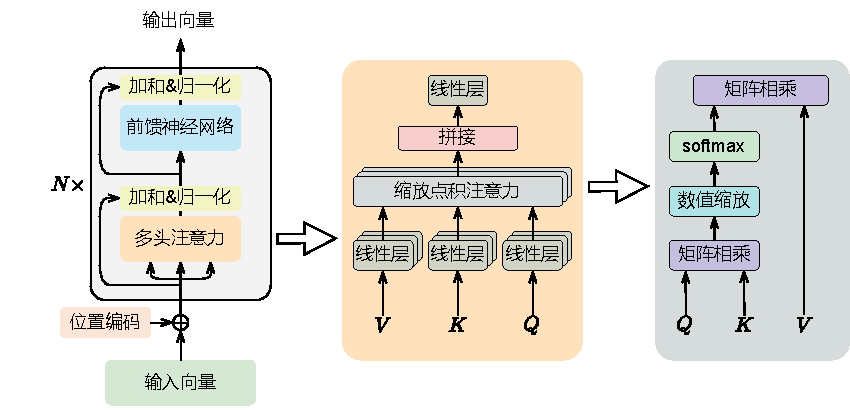
\includegraphics[width=1\linewidth]{figures/chap2/transformer.pdf}
   \caption{Transformer编码器示意图}
   \label{transformer}
\end{figure}

在预训练阶段,BERT利用文档级别的大规模英文文本语料集,其包括英文维基百科数据和BooksCropus语料库,执行如下两个预训练任务:

(1)遮掩语言模型(Masked Language Model,MLM):受完形填空的启发,该任务随机选取15\%已切分的WordPiece~\cite{wu2016google}输入序列中的词元进行遮掩,并使用BERT预测被遮掩的词元。但该遮掩训练方式与微调阶段存在不一致。因此,基于此15\%被选中的词元作进一步操作:保留其中80\%词元的遮掩操作,取消其中10\%词元的遮掩操作,并将剩下的词元随机替换成其他词元。通过提供预测词元的不确定性,促使模型更多地学习到全局上下文信息。

(2)下一句预测(Next Sentence Prediction,NSP):以文本对方式构建该任务输入,表示为“$[CLS]+S_{A}+[SEP]+S_{B}+[SEP]$”,其中$[CLS]$和$[SEP]$为特殊词元。该任务仅保留语料数据中一半句子的真实下一句作为$S_{B}$,另一半句子的$S_{B}$从语料集中随机选取得到,其旨在通过特殊词元$[CLS]$预测$S_{B}$是否被随机替换。通过此任务的训练,提升BERT模型在自然语言推理和问答等任务上的语言理解能力。

在下游任务微调阶段,根据任务的特点,选择单个文本或文本对输入到预训练BERT模型中,并叠加额外的设计模块进行训练损失微调。在事件检测任务中,Yang等人~\cite{yang2019exploring}首先利用BERT模型获取各个词的特征表示并构建多分类器进行事件类型的建模。Wang等人~\cite{wang2019adversarial}将DMCNN~\cite{chen2015event}模型中的CNN替换成BERT,保留其动态池化操作,构建对应的DMBERT进行事件预测。Liu~\cite{liu2020event}等人将事件检测问题转化为机器阅读理解任务,其简单地构建了一个特殊查询命令“[EVENT]”并和待抽取文本进行串接输入到BERT中,对于每个单词使用多分类的方法建模其对应的事件类型信息。类似地,Du等人~\cite{du2020event}设计了四类静态的问答模版用于事件检测,包括“what is the trigger”、“trigger”、“action”和“verb”,并同样使用多分类器进行事件类型的建模预测。与Liu等人~\cite{liu2020event}和Du等人~\cite{du2020event}不同,一些研究考虑显示地在预训练语言模型中利用事件类型的语义知识,深度建模其与待抽取上下文间的交互关系。例如,Li等人~\cite{li2020event}为了在BERT中利用到不同事件类型名称本身的语义信息,其将事件检测任务转化为多轮问答。具体地,首先设计固定的问题模版预测事件触发词的开始和结束位置,然后枚举所有的预定义事件类型并和已预测的触发词文本、触发词位置进行串接,根据特殊字符$[CLS]$进一步确定所属的事件类型。该方法不依赖预定义的事件类型数目,可扩展到新的事件类型预测,在零样本和少样本场景下同样表现出良好的性能潜力。Wang等人~\cite{wang2022query}使用事件类型名称和高频原型触发词作为对应事件类型的描述,然后枚举所有的事件类型描述并分别与待抽取文本串接,利用二分类方式建模对应的事件触发词。进一步,在相同的框架下,Wang等人~\cite{wang2022art}丰富了事件类型的描述模版,增加了事件定义、相关的事件要素类型、自动学习的软模版和人工构建的事件模版等信息。

进一步,一些工作基于BERT深入研究事件检测模型的鲁棒性、知识增强和预测模式等问题,以更好地挖掘预训练语言模型的潜力。例如,现有事件检测建模过于依赖词法信息,欠缺良好的上下文建模能力,从而导致在预测罕见或未出现的触发词时性能下降明显~\cite{lu2019distilling}。针对该问题,Liu等人~\cite{liu2020does}提出了两种上下文遮掩策略,以提升BERT模型在事件检测任务上的鲁棒性。第一种为句内策略,旨在提升模型学习句内上下文中的显著语义信息。具体地,固定已训练的事件检测模型的参数,其首先只遮掩候选触发词并使用遮掩向量作为查询向量计算对应的上下文注意力分布$\boldsymbol{\alpha}_{u}$,然后随机采样多种遮掩序列同样计算其上下文注意力分布。如果其中存在遮掩序列能够提升模型的预测结果,则以对应的上下文注意力分布作为训练目标,减少其与$\boldsymbol{\alpha}_{u}$的方差。第二种为句间策略,其基于单词分布假设~\cite{harris1970distributional},增加相同事件类型的触发词被遮掩后的上下文间的相似度,反之则减少对应的上下文间的相似度。类似地,Tong等人~\cite{tong2020improving}也观察到现有方法在预测罕见和未出现的事件触发词时性能表现不佳,并将其归因于数据集中存在的事件类型长尾分布。为了解决该问题,其基于知识蒸馏技术,将根据词义获取的开放域触发词知识用于提升对这两类事件触发词的识别。具体地,首先使用WordNet~\cite{miller1990introduction}数据库从词义的角度实现对New York Times~\cite{sandhaus2008new}语料库的快速大规模标注,以获取开放域触发词知识。然后,构建知识蒸馏框架,促使教师网络和学生网络在监督数据集和大规模标注数据集上的预测概率均保持相似,从而实现开放域触发词知识的迁移。其中,在教师网络输入文本中使用两个特殊字符标注触发词的边界信息,而在学生网络输入文本中则遮掩对应的触发词,从而促使基于上下文信息的学生网络从教师网络中更好地学习识别触发词的能力。Liu等人~\cite{liu2022saliency}使用基于BERT训练的事件检测模型量化区分事件类型的潜在模式并根据模式的不同采取相应策略增强预测性能。具体地,利用可解释领域的积分梯度算法(Integrated Gradient)\cite{sundararajan2017axiomatic},计算文本中每个单词$w_{i}$对于事件预测的贡献值,具体如下:
\begin{equation}
\boldsymbol{\alpha}_{w_i}=\left(\boldsymbol{x}_i-\boldsymbol{x}_i^{\prime}\right) \times \int_{\alpha=0}^1 \frac{\partial \mathcal{L}\left(t ; \boldsymbol{X}^{\prime}+\alpha \times\left(\boldsymbol{X}_s-\boldsymbol{X}^{\prime}\right)\right)}{\partial \boldsymbol{x}_i} d \alpha
\end{equation}
其中$\boldsymbol{x}_i$为$w_{i}$由BERT编码得到的特征表示,$\boldsymbol{X}_s$为文本中所有单词对应的特征表示组成的序列,
$\boldsymbol{X}^{\prime}$为对应于$\boldsymbol{X}_s$的零向量序列,$\boldsymbol{x}_i^{\prime}$为$\boldsymbol{X}^{\prime}$序列中第$i$个向量,$t$为预测的事件类型的独热向量表示。

基于此,进一步归一化得到的预测贡献值,
% \begin{equation}
% \alpha_{w_i}=e^{\left\|\boldsymbol{\alpha}_{w_i}\right\|_2} / \sum_{n=1}^N e^{\left\|\boldsymbol{\alpha}_{w_n}\right\|_2}
% \end{equation}
% 其中$\|\|$为$L_{2}$范数。
并根据每个单词的贡献值,计算不同事件类型的触发词在整体训练集中的平均贡献。然后,设置阈值且根据每个事件类型触发词的平均贡献将其划分为触发词依赖的事件或上下文依赖的事件。对于前者,构建基于BERT的事件检测模型并在输入中使用额外的单词显著贡献向量来标记各个单词的贡献值信息,辅助模型聚焦于具备高贡献值的单词进行建模。对于后者,构建另一个基于BERT的事件检测模型并在输入中串接具有高贡献值的上下文片段,辅助模型更好地利用相关上下文信息。在测试阶段,集成此两个事件检测模型的预测,得到最终的检测结果。
% 针对BERT由于输入长度的限制而无法在事件检测中编码更多的跨句信息,Veyseh等人~\cite{veyseh2021modeling}基于强化学习算法REINFORCE自动学习从跨句信息中选择重要的上下文信息参与到BERT编码中。具体地,枚举选择不同句子组成的上下文,考虑从BERT建模事件检测的性能、选择上下文与目标句子的语义相似性和实体共指的数量等多个角度评估对应的奖励值,从而指导算法参数的更新。

此外,存在一些研究工作基于自回归预训练语言模型进行事件检测的数据增广。例如,Veyseh等人~\cite{veyseh2021unleash}使用GPT-2~\cite{radford2019language}生成训练数据。为了降低生成数据中的噪音信息,其设计了教师-学生网络。教师网络使用高质量数据集进行训练得到,而学生网络则同时使用高质量数据和生成数据进行训练,并保持与教师网络的知识一致性。

近年来,以ChatGPT、PaLM~\cite{chowdhery2023palm}和LLaMA~\cite{touvron2023llama}为代表的大语言模型(Large Language Models,LLMs)在自然语言处理的很多研究领域取得了令人印象深刻的性能表现。在事件检测任务上,一些研究者基于ChatGPT进行了相关性能的评估。例如,Li等人~\cite{li2023evaluating}基于零样本场景评测了ChatGPT在事件检测任务上的性能。具体地,其设计的输入提示模版包括对于任务的描述、预定义的事件类型集合、待抽取的文本内容和形式化的输出格式要求。Gao等人~\cite{gao2023exploring}丰富了输入提示模版的内容,一方面其扩充了对于各个预定义事件类型的详细描述,同时给出了正确样例和错误样例的输入输出信息。基于此,选取测试集中部分样例进行了性能评测。进一步,Han等人~\cite{han2023information}设计了与Li等人~\cite{li2023evaluating}相似的提示模版,并引入情景学习(In-Context Learning,ICL)\cite{brown2020language}和思维链(Chain-Of-Thought,COT)\cite{wei2022chain}技术,提升了少样本场景下ChatGPT在事件检测任务上的性能。具体地,在原有提示模版的基础上,添加5个从训练集中随机采样的训练数据的文本信息和对应的正确事件检测结果作为示例,从而构建出5-shot ICL提示模版。对于5-shot COT提示模版,其关于事件检测的解释过程由人工进行构造。虽然这些研究采取了提供负样例、ICL和COT等不同策略提升性能,但评估结果均表明ChatGPT在事件检测任务上的性能仍与现有监督模型存在明显差距。

\section{给定实体提及的事件要素抽取}
\label{section2_2}
事件要素抽取(Event Argument Extraction)旨在根据事件检测得到的事件触发词和事件类型信息,进一步识别事件中存在的事件要素以及对应的事件要素类型。识别得到的事件要素作为结构化的语义信息,广泛应用于多种下游任务~\cite{wen2021resin,wu2022cross,fung2023deepmaven,liu2023covid}。

现有的事件要素抽取任务存在两种不同的定义方式。第一种定义方式主要基于自动内容提取项目(Automatic Content Extraction,ACE)\footnote{http://projects.ldc.upenn.edu/ace/}。该项目在评估设置中将实体提及的识别和事件要素抽取分离,因此在事件要素抽取中可以直接利用到实体提及的标签信息。具体地,给定待抽取文本、事件触发词和事件类型,本定义下的事件要素抽取将文本中已知存在的实体提及均视作候选事件要素,旨在识别出所有作为事件要素出现的实体提及,并给出对应的预定义事件要素类型。由于ACE项目聚焦于句子级别的信息标注,待抽取文本一般为单个句子。随着近年来文本信息朝着复杂化方向演变,出现了以RAMS~\cite{ebner2020multi}和WikiEvents~\cite{li2021document}为代表的文档级别事件要素抽取数据集,其将实体提及的识别包含在事件要素抽取任务中。为了更好地研究适合不同文本级别的事件要素抽取模型,最近的一些事件要素抽取方法~\cite{ma2022prompt}给出了不同的定义方式。具体地,给定由单个句子或多个句子组成的待抽取文本、事件触发词和事件类型,该定义下的事件要素抽取旨在识别出每个事件要素的文段范围以及对应的预定义事件要素类型。与第一种定义不同的是,其要素类型的预测范围特定于给定事件类型,而非数据集中所有预定义的要素类型。

基于定义方式的不同,相应事件要素抽取研究工作的建模方式也存在较大差异。因此,本章主要介绍基于第一种定义方式的技术发展情况,其相关工作均根据ACE项目或类似的定义进行建模和评估。而第二种定义方式下的事件要素抽取技术将在下一章节进行梳理。

与事件检测任务相似,早期的事件要素抽取方法同样基于人工设计的事件模式或特征进行构建。其中,基于事件模式的方法结合词性标注结果和候选事件模式,匹配出对应的事件要素信息~\cite{cao2018including}。而基于特征的方法主要使用词法特征和句法特征~\cite{li2013joint}。词法特征一般包括单词的不同形态,如其完整形式和小写形式,以及词性标注信息等。而句法特征一般从依存句法解析结果中获取,表示为单词间依存关系形成的句法树。更具体地,给定一个单词,其主要句法特征信息一般为该单词在句法树中的深度、存在句法依存关系的词及对应的依存关系标签等。

进一步,虽然在本章梳理的事件要素抽取任务中,事件要素分布范围限定在单个句子,但存在一些研究工作基于更大范围的文本利用全局特征增益单个句子的要素抽取性能,如跨文档、跨句子和跨事件中的实体提及、事件要素和语义信息等。例如,Ji等人~\cite{ji2008refining}利用相同实体在相关文档内的相同事件中通常以相同要素类型出现的一致性规律作为全局信息依据,辅助局部的事件要素抽取。在此基础上,Liao等人~\cite{liao2010using}进一步考虑相同实体在
不同类型的事件中要素类型呈现的一致性。例如,在ACE2005数据集中,$Attack$(攻击)事件中以$Target$(目标)要素类型出现的实体存在较大概率在$Injure$(受伤)事件和$Die$(死亡)事件中以$Victim$(受害者)要素类型出现。不同于Ji等人~\cite{ji2008refining}和Liao等人~\cite{liao2010using}利用全局信息辅助调整局部抽取结果,Hong等人~\cite{hong2011using}直接使用全局的跨事件实体类型间的关系作为参与要素分类的特征。具体地,其基于ACE2005数据集的统计结果发现大多数具有相同实体类型的实体提及出现在相同类型的事件中,且进一步观察到这些实体提及中的大多数在事件中仅以少数几种要素类型出现。为了利用实体类型与事件类型和要素类型的一致性,其设计了事件类型、实体类型、领域内共现实体类型等特征,以用于句内要素识别的二分类预测和要素类型的多分类预测。此外,Liao等人~\cite{liao2011acquiring}使用Latent Dirichlet Allocation(LDA)\cite{blei2003latent}主题模型得到每个文档的主题分布信息,然后将该全局信息作为特征应用到要素抽取中。

近年来,基于神经网络的事件要素抽取方法成为主流,其克服了模式构建和特征工程的困难。接下来,本章根据神经网络架构的类型,对这些方法进行总结。

\subsection{基于卷积神经网络的方法}

与图\ref{dmcnn}所示的DMCNN模型类似,Chen等人~\cite{chen2015event}也将其应用到事件要素抽取任务上。在卷积层部分,其与事件检测中使用的DMCNN模型相同。但在动态池化部分,考虑到相同候选要素可能在不同的事件中以不同的要素类型出现,其在图\ref{dmcnn}的两部分划分的基础上,基于候选要素的位置作进一步划分,以根据事件触发词和候选要素建模到更加关键的信息。然后,利用划分为三段子文本的特征表示分别进行最大池化并拼接,以用于事件要素的预测。Wang等人~\cite{wang2019hmeae}基于DMCNN,进一步考虑不同要素类型间存在的语义概念的相关性。例如,要素类型$Buyer$(买家)和$Seller$(卖家)在抽象的概念层级中均与概念$Person$(人物)和$Org$(机构)存在关联,因此这两个要素类型间的语义概念相关性要强于其他和这两个概念没有关联的要素类型。为了利用这种语义概念信息,其在DMCNN的基础上进一步构建了层次模块化注意力。对于给定的要素类型和每个关联概念的向量表示,分别计算每个单词对应的注意力得分,并进一步得到每个单词基于所有关联概念的平均注意力得分,以权重求和对应的特征表示,从而获取给定要素类型的上下文表示向量。在计算每个要素的预测概率时,将对应的上下文表示向量与DMCNN编码表示进行拼接,以利用到相关的语义概念信息。

\subsection{基于循环神经网络的方法}
Nguyen等人~\cite{nguyen2016joint}最早在事件要素抽取中使用RNN。其构建预训练词向量、实体类型向量和二元依存句法关系向量作为输入,使用双向GRU网络获取文本中每个单词的特征表示。为了捕捉事件检测和事件要素抽取结果的相关性,其根据文本中单词的顺序依次进行预测。具体地,当预测到特定的单词时,首先判断其是否为事件触发词。若该单词为事件触发词,则在预测候选事件要素的类型时,考虑利用之前已经预测得到的事件类型和要素类型信息。进一步,Sha等人~\cite{sha2018jointly}考虑将句法信息融合到双向LSTM网络中。具体地,对于不同的依存句法关系及其相应的逆关系,设置不同的权重值,并基于此修改LSTM隐藏层特征表示的计算:
\begin{equation}
    \boldsymbol{h}_t=\boldsymbol{o}_t \odot \tanh \left(\boldsymbol{c}_t\right)+\boldsymbol{d}_t \odot\left(\frac{1}{\left|S_{i n}\right|} \sum_{(i, p) \in S_{i n}} a_p \boldsymbol{h}_i\right)
\end{equation}
其中$\boldsymbol{o}_t$和$\boldsymbol{c}_t$分别为LSTM的输出门控向量和记忆单元向量,$S_{i n}$中的每个元素$(i, p)$表示与第$t$个单词存在依存句法关系的单词顺序索引和对应的关系类型索引,$a_{p}$为对应的关系权重值,$\boldsymbol{d}_{t}$用于控制句法信息的过度影响,其基于第$t$个单词的输入向量和第$t-1$个单词的隐藏层特征表示学习得到。此外,该方法在要素分类中考虑同时建模不同要素间的交互。为此,其首先利用线性层得到任意候选要素间的交互向量。
% \begin{equation}
%     \boldsymbol{T}_{i j}=\tanh \left(\boldsymbol{W}_d\left[\boldsymbol{h}_i, \boldsymbol{h}_j\right]+\boldsymbol{b}_d\right)
% \end{equation}
% 其中$\boldsymbol{W}_d$和$\boldsymbol{b}_d$为训练参数。
然后,给定每个候选要素,对其所有交互向量进行逐元素最大池化操作,以捕捉最显著的交互信息。同时,基于交互向量建模不同候选要素间的注意力权重和上下文要素表示。
% \begin{equation}
%     A_{i j}=\operatorname{softmax}\left(\tanh \left(\boldsymbol{W}_a \boldsymbol{T}_{i j}+b_a\right)\right)
% \end{equation}
% \begin{equation}
%     \boldsymbol{F}_A=\boldsymbol{A} \boldsymbol{H}^{\top}
% \end{equation}
% $\boldsymbol{W}_a$和$b_a$为学习参数,$\boldsymbol{H}$为所有候选要素特征表示依次堆叠得到的矩阵。
最后,串接每个候选要素的最大池化交互向量、上下文要素表示、编码特征表示和事件触发词的编码特征表示,以进行要素类型的预测。

此外,Nguyen等人~\cite{nguyen2019one}利用RNN编码得到的特征表示同时建模实体提及识别、事件检测和事件要素抽取任务,构建多任务学习损失进行训练,实现不同任务间的知识共享和隐式依赖捕捉,以提升事件要素抽取任务的性能。在建模过程中,其沿用了Nguyen等人~\cite{nguyen2016joint}的方法,按照单词顺序依次预测事件触发词和事件要素,并在要素预测时利用之前步骤预测的相关要素类型和事件类型信息。

% 在输入部分,构建预训练词向量、词性、组块和句法依赖关系的二元表示向量,使用双向GRU进行编码。然后,与Nguyen等人~\cite{nguyen2016joint}的研究工作类似,其按照单词顺序依次建模预测事件触发词和事件要素信息。具体地,在建模事件要素类型分类时,串接事件触发词和候选要素的上下文编码表示以及触发词对应事件类型、候选要素对应实体类型、触发词和候选要素之间的最短依存句法路径、候选要素在之前步骤预测的相关要素类型和事件类型信息~\cite{nguyen2016joint}等,使用多分类器得到相应的要素类型概率分布。

\subsection{基于预训练语言模型的方法}

第一种定义方式下的事件要素抽取方法主要使用的预训练语言模型为BERT。例如,Wang等人~\cite{wang2019hmeae}构建了事件要素抽取的基线模型DMBERT,其将DMCNN中的卷积层替换为BERT~\cite{devlin2019bert}。进一步,Wang等人~\cite{wang2019hmeae}在其提出的HMEAE框架中,使用DMBERT替代DMCNN获取文本编码表示。在DMBERT的基础上,Xi等人~\cite{xiangyu2021capturing}引入Nguyen等人~\cite{nguyen2016joint}用于存储已经预测得到的事件类型和要素类型信息而设计的二元记忆矩阵,构建可以利用跨事件信息的BERT(Inter)模型。同时,Xi等人~\cite{xiangyu2021capturing}参照Sha等人~\cite{sha2018jointly}建模不同事件要素间的交互向量和上下文要素表示,构建可以捕捉事件内不同事件要素关联性的BERT(Intra)模型。

然而,BERT(Intra)隐式地构建事件要素间交互的方式无法直接使用其他要素预测结果,且要素类型的本身语义信息也未得到充分利用。基于此,Xi等人~\cite{xiangyu2021capturing}将事件要素抽取转化为序列到序列的建模问题,其中输入序列为标注了特定事件触发词信息的句子文本,输出序列为文本中候选要素对应的要素类型序列。为了双向利用事件内不同事件要素的类型预测语义信息,其使用编码器-解码器框架并针对性地提出了实体级别的双向循环解码架构。具体地,在编码器的输入文本尾端融合给定事件触发词的事件类型信息,并利用BERT获取每个单词的特征表示。而在解码器中,根据事件触发词和待抽取的实体提及位置信息,对编码器输出的特征表示使用DMCNN~\cite{chen2015event}中的动态池化操作获取实例的整体特征表示。另一方面,使用CNN编码包含了每个单词在之前序列预测中获取的要素类型标签向量,从而融合已预测的事件要素信息,并同样利用最大池化操作得到其中最显著的事件要素信息的特征表示。然后,基于这两部分的特征表示,使用多分类器进行事件要素类型的解码。进一步,该模型在解码部分构建了正向和逆向两个不同的建模过程,在推断时使用双向建模得到的事件要素信息的特征表示参与最终的事件要素预测。

\section{未给定实体提及的事件要素抽取}
\label{no_entity}
如上一章节所述,最近一些研究工作将事件要素抽取任务定义为旨在同时识别出事件要素的文段范围和要素类型,其抽取过程未使用实体提及识别任务的结果。因此,本章调研未给定实体提及的事件要素抽取的研究现状。随着基于Transformer架构的预训练语言模型技术的不断成熟,其预训练-微调模式已成为未给定实体提及的事件要素抽取方法的主流选择。其中,BERT、RoBERTa~\cite{liu2019roberta}和BART~\cite{lewis2020bart}为本章介绍的方法中常用的预训练语言模型。

RoBERTa使用了与BERT完全相同的模型结构,但在预训练设置上提出了如下改进:(1)在更大规模的英文语料库上进行预训练,相比于BERT使用的数据量扩增了10倍有余。(2)针对更大规模的训练数据,相应地将训练时的批数据大小增加到8000,远超BERT设置的256。(3)直接串联连续的多个句子作为输入,并移除BERT预训练中构建的NSP任务。(4)在MLM预训练任务中采用动态遮掩替代BERT中的静态遮掩设置。在BERT的静态遮掩设置中,被遮掩的WordPiece词元一旦确定,则在整个预训练过程中不再改变。而RoBERTa则将初始训练语料复制10份,分别随机选择不同的WordPiece词元进行遮掩,然后在训练的不同轮数使用经过不同遮掩选择得到的输入序列。

BART(Bidirectional and Auto-Regressive Transformers)为序列到序列预训练语言模型,与BERT和RoBERTa不同,其使用了与Transformer~\cite{vaswani2017attention}相同的编码器-解码器架构。BART本质上为一个将经过噪音信息破坏的文本还原成对应初始序列信息的去噪自编码器。在预训练中,BART主要使用了如下的噪音引入方式:(1)遮掩词元:与BERT在MLM预训练任务中的设置相同,随机采样文本中的词元进行遮掩处理。(2)删除词元:随机采样文本中的词元进行删除处理,提升模型感知缺失词元位置信息的能力。(3)填充文本:采样不定长度的词元片段进行遮掩,该方式受Joshi等人在SpanBERT~\cite{joshi2020spanbert}预训练语言模型中的设置启发。具体地,采样长度服从泊松分布(参数$\lambda$为3)的词元片段进行遮掩处理。当长度为0时,则在文本中直接插入代表遮掩处理的特殊词元“[MASK]”。该方式使得BART模型能够感知缺失的词元片段中的词元数量。(4)旋转文本:随机选择文本中的一个词元,以该词元为界将整个文本划分为两部分,并旋转对调这两部分文本段,使得旋转后整个文本的开始词元为选择的词元。该设置可以提升模型对于原始文本的开头信息的识别。(5)置换句子:随机置换文本中的句子顺序。基于上述的文本破坏方式,构建相应的重建文本损失进行BART模型的预训练。BART模型广泛应用在序列生成、序列分类和词分类等任务中。

基于预训练语言模型,可进一步将现有未给定实体提及标注的事件要素抽取方法总结为如图\ref{four_cls}所示的四种类型。在该图中,
“computer”以要素类型$Artifact$(人工制品)参与到$Transfer-Ownership$(转让所有权)事件中。接下来,分别介绍各自类型的相关工作和方法特点。

\begin{figure}[htp]
   \centering
   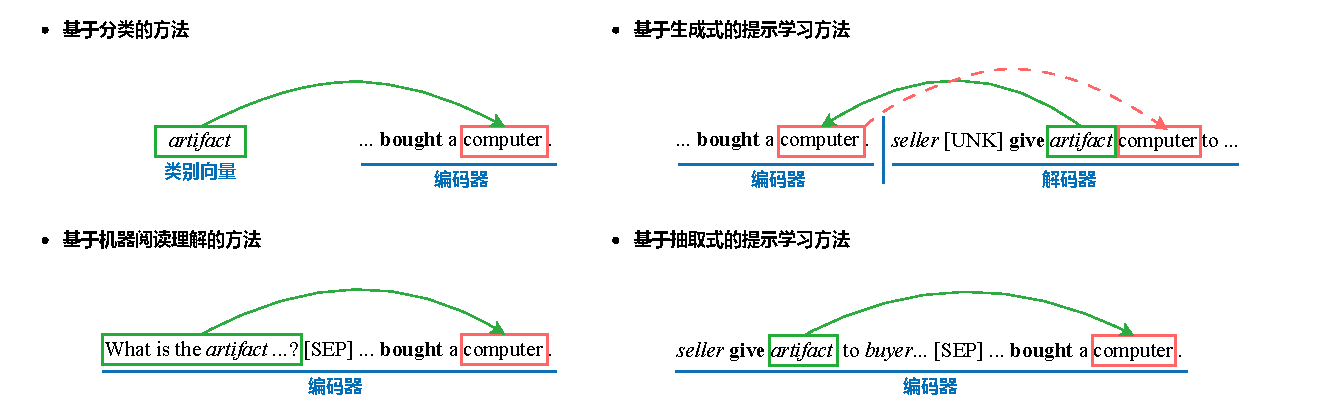
\includegraphics[width=1\linewidth]{figures/chap2/four_cls.pdf}
   \caption{四类事件要素抽取方法示意图}
   \label{four_cls}
\end{figure}

\subsection{基于分类的方法}

基于分类的方法使用传统的分类方式,构建随机初始化的分类器进行事件要素的预测。Ma等人~\cite{ma2020resource}利用预训练语言模型获取能够感知触发词信息的序列上下文表示,并进一步设计了融入依存句法结构信息的Transformer架构,得到融合句法信息的编码表示,最后使用多分类器同时完成要素文段范围和类型的建模。具体地,其首先使用BERT编码待抽取文本,并利用BERT输入中的分隔向量(segment embedding)区分对应词是否为事件触发词。对于每个词,在其BERT输出的编码表示基础上,均串接触发词和触发词对应的事件类型等信息,以增强对于事件信息的感知。然后,根据文本的依存句法解析结果,修改Transformer中的多头自注意力机制,将每个词注意力计算中的键和值限制为与其存在依存句法关系的词,从而使得其聚焦句法关联词间的自注意力建模。最后,结合预定义要素类型和BIO标注策略,利用多分类器同时完成对事件要素的文段和类型的抽取。与Ma等人~\cite{ma2020resource}直接使用序列标注建模的方式不同,一些研究者将事件要素抽取分解为子任务依次解决。例如,Zhang等人~\cite{zhang2020two}将文档级别事件要素抽取拆解为要素头单词识别和基于头单词的文段扩充两个子问题。在要素头单词识别中,对于要素类型$r$,利用特定于$r$的双仿射注意力机制(Biaffine)\cite{dozat2018simpler}参数建模候选词作为该要素类型出现的概率:
\begin{equation}
    \textrm{Pr}_r(t, c)=\frac{\exp \textrm{Biaffine}_r\left(\boldsymbol{e}_t, \boldsymbol{e}_c\right)}{\sum_{c^{\prime} \in \mathcal{C} \cup\{\epsilon\}} \exp \textrm{Biaffine}_r\left(\boldsymbol{e}_t, \boldsymbol{e}_{c^{\prime}}\right)}
\end{equation}
其中$\boldsymbol{e}_t$和$\boldsymbol{e}_c$为事件触发词和候选词经BERT编码后得到的特征表示,$\mathcal{C}$为候选词集合,$\epsilon$表示要素类型$r$不存在对应要素。而在获取头单词后,根据设置的最大要素文段长度,枚举所有可能的候选左边界和右边界词。然后,将基于头单词的文段扩充子问题转化为寻找包含该头单词的左右边界词问题,并视每个候选边界词为一个类别,构建两个多分类任务分别建模。同样地,Xu等人~\cite{xu2022two}将文档级别事件要素抽取转化为要素边界识别和要素类型分类两个子任务依次进行建模。在要素边界识别任务中,使用两个不同的BERT编码器捕捉局部和全局上下文信息。其中,局部信息的编码通过遮掩跨句词间的注意力计算得到。进一步,为了在局部信息中融入更加丰富的语义结构知识,其基于抽象语义表示(Abstract Meaning Representation,AMR)\cite{banarescu2013abstract}的解析结果,使用GCN对于局部编码表示进行语义关联信息的聚合。最后,基于门控机制融合包含了语义结构知识的局部信息和文档全局信息,并使用两个二分类损失构建要素边界的识别。而在要素类型分类中,同时使用触发词、事件类型、识别出的要素以及要素与触发词间的交互等信息进行要素类别的判断。此外,Liu等人~\cite{liu2023enhancing}将事件要素抽取转化为基于枚举文段的分类问题。具体地,其使用BERT或RoBERTa模型联合编码事件信息、待抽取文本和事件相关的要素类型信息,并对于给定的枚举文段,使用同时与该文段和事件触发词存在相关性的上下文和要素类型信息作为其整体表示。在此基础上,一方面根据对应的边界表示构建二分类边界损失,另一方面融合整体表示、边界表示和事件触发词表示等信息,构建事件要素类型的多分类损失。

\subsection{基于机器阅读理解的方法}

本类方法为每个要素类型构建相应的问题,将抽取对应要素转变为机器阅读理解(Machine Reading Comprehension,MRC)\cite{rajpurkar2016squad}问题,其能够同时获取要素的边界和类型信息,并利用到要素类型本身的语义知识。Du等人~\cite{du2020event}探索了三种不同的要素类型问题模版,包括只使用要素类型名称、结合要素类型名称与对应语义类型的疑问词、结合ACE项目中关于要素类型的标注指南与对应疑问词。然后,使用BERT对待抽取文本和问题模版进行联合编码,并参照传统的MRC方法构建要素开头和要素结尾的查询向量,使用softmax归一化建模文本中每个词分别为要素开始词和要素结尾词的概率。由于给定要素类型可能不存在或存在多个事件要素,在要素边界推断时需人为设置预测阈值。为此,其进一步根据验证集设计启发式算法,以动态决定划分要素文段和非要素文段边界概率值的最佳阈值。同样地,Li等人~\cite{li2020event}设计了包含事件触发词、事件类型和待抽取的要素类型等信息的模版作为MRC中的对应问题。为了抽取可能存在的多个事件要素,其根据每个词的编码表示构建BIO的三分类器,以替代Du等人~\cite{du2020event}采用预测阈值的做法。与Du等人~\cite{du2020event}和Li等人~\cite{li2020event}基于规则模版构建问题不同,Liu等人~\cite{liu2020event}利用无监督问题生成技术,获取与待抽取文本上下文和主题相关的自然语言表达的问题,以提升MRC模型获取答案的能力。其无监督问题生成主要包括两个部分:问题主题生成和问题上下文生成。问题主题生成与Du等人~\cite{du2020event}的设置相似,通过要素类型的语义类型使用不同的疑问词作为问题开端。而在问题上下文生成中,设计两个不同的编码器-解码器架构,以分别学习陈述性文本映射到问题描述和对应的相反映射。进一步,构建由大规模陈述性文本和未对齐的问题组成的数据语料,利用领域内自编码、去噪自编码和跨领域在线还原翻译任务进行训练。最后,使用将陈述性文本映射到对应问题的编码器-解码器模型生成待抽取文本对应的问题上下文。Zhou等人~\cite{zhou2021role}根据要素文段识别和要素类型识别分别构建两个对偶的MRC任务,通过参数共享和联合训练,实现相互协作,以提升建模性能。具体地,基于BERT分别编码待抽取文本、由要素文段和要素类型转换的问题,并利用流动注意力模块~\cite{seo2016bidirectional}实现问题表示和待抽取文本表示的交互。

进一步,一些研究利用MRC技术解决文档级别事件要素抽取带来的新问题与挑战。例如,Liu等人~\cite{liu2021machine}为了解决文档中存在的事件数据稀疏问题,利用MRC实现两种不同的数据增广。一方面,利用机器阅读理解、语义角色标注~\cite{atkins2003contribution}和事件要素抽取的跨任务数据集进行MRC模型的预训练,实现相似任务中隐式知识的传递。另一方面,使用预训练后的模型对无标注信息的文档进行事件要素信息的标注,以生成事件要素抽取任务中的更多数据实例。Wei等人~\cite{wei2021trigger}考虑到文档数据中事件要素可能分布在不同句子中,使得模型无法较好地捕捉事件触发词与要素间的长距离依赖以及事件要素间的隐式关联。为此,其在MRC模型中引入知识蒸馏技术,以提升模型在长范围文本场景下的事件内部推理和依赖知识建模能力。具体地,在其知识蒸馏框架中,对于每个要素类型,在教师网络的输入中引入事件内其他要素文段和类型信息,并使用MRC进行对应要素文段的建模。而在学生网络中,同样构建MRC抽取要素文段。基于此,从特征表示和预测概率分布两种角度将教师网络中引入的相关要素知识迁移到学生网络中。

% 进一步,采用输入中包含不同相关要素信息的多教师网络策略以提供学生网络学习到多视角知识,并基于课程学习技术逐步增加学生网络与教师网络输入不同的训练实例比例,以增强学生网络的学习效率。

此外,存在研究工作利用序列到序列框架直接生成对应的要素文段,以替代从文本中建模要素文段的范围。例如,Lu等人~\cite{lu2023event}首先构建问题生成模型,为每个要素类型获取包含了其他要素信息的问题,然后基于BART或T5~\cite{raffel2020exploring}模型生成所有归属该要素类型的要素文段。其问题生成模型同样基于BART或T5构建,输入序列为待抽取文本,对应输出序列则融合了ACE项目中关于目标要素类型的标注指南和待抽取文本中存在的其他要素文段信息。

% 采取了与Liu等人~\cite{liu2020event}类似的方法,以生成与待抽取文本相关的动态模版。为此,构建输入序列为待抽取文本,对应输出序列则融合了ACE项目中的关于目标要素类型的标注指南和待抽取文本中存在的其他要素文段信息,同样使用BART或T5进行建模。

\subsection{基于生成式的提示学习方法}

本类方法构建提示模版,利用序列到序列模型生成待抽取的事件要素信息,其相比基于机器阅读理解的方法,能够更加直接地同时抽取多个具有相同要素类型的事件要素。Li等人~\cite{li2021document}将文档级别事件要素抽取建模为基于提示模版进行填空的条件生成任务。其使用的提示模版为数据标注时参照的事件本体模版,并将模版中具体的要素类型名称替换为特殊占位符,即挖空操作。进一步,将经过挖空的提示模版和文本串接后输入到BART模型的编码器中,并在解码器中依次建模已完成要素文段填空后的提示模版序列。然后,比对填空的文段内容和对应被挖空的要素类型名称,实现要素信息的抽取。若挖空槽位的所属要素类型对应文本中多个要素文段,则在解码时使用“and”进行串联。Zeng等人~\cite{zeng2022ea2e}使用了和Li等人~\cite{li2021document}完全相同的模型架构和提示模版进行文档级别的事件要素抽取。不同的是,其在此基础上对于每个输入文本同时构建一个标注了相邻事件要素类型标签的信息增广文本,并通过对齐这两种输入文本中事件要素的编码表示,使得模型更好地感知跨事件要素的语义一致性。

类似地,Hsu等人~\cite{hsu2022degree}使用序列生成模型构建适用于不同级别文本的事件要素抽取。其与Li等人~\cite{li2021document}的研究工作相比,主要存在以下不同:(1)在构造提示模版时融合了更丰富的事件信息,包括事件类型定义和与事件语义密切相关的关键词。(2)在对事件提示模版进行挖空时,使用自然语言词汇如“some attacker”、“some organization”等替代Li等人~\cite{li2021document}使用的特殊词符进行占位。该设计使得模型可以更好地学习到要素类型的语义信息和事件整体结构信息。(3)基于人工设计进行事件提示模版的构造,未直接利用数据集中的事件本体模版知识。在序列生成模型的基础上,Hsu等人~\cite{hsu2023ampere}进一步利用AMR语义图知识。其将文本的AMR语义解析图转化为线性序列,并编码表示为若干向量表示,添加到模型Transformer架构的键向量和值向量中,从而实现结构化图知识与自然语言文本的异质融合。

进一步,Du等人~\cite{du2022dynamic}研究当文档中存在较多事件时,在序列生成模型中利用已预测的跨事件知识进行信息增益。在预测目标事件时,使用预训练的文本相似度衡量模型S-BERT~\cite{reimers2019sentence}检索出最相关的已预测事件序列,并作为额外的记忆知识和文本以及事件提示模版串接输入到生成模型的编码器中,为目标事件的要素抽取提供跨事件信息。而当预测下一个事件的要素时,根据当前目标事件要素抽取结果转化的事件序列信息将同样参与到相似度检索中,从而不断丰富待检索的事件知识。进一步,Ren等人~\cite{ren2023retrieve}研究在序列生成框架中利用多种检索增强策略提升事件要素抽取性能,包括上下文一致检索、模式一致检索和自适应混合检索。其中,上下文一致检索策略与Du等人~\cite{du2022dynamic}采用的方法相似,模式一致检索策略利用事件类型标签进行检索查询,而最后一种策略则采用连续空间中的伪示例采样进一步提升序列生成模型的类比能力。

% 此外,Zhang等人~\cite{}使用序列生成模型建模事件要素抽取的同时,利用跨数据集中的重叠知识增强模型在目标数据集的性能。训练过程可分为两大阶段:重叠知识学习阶段和特定知识学习阶段。在第一阶段中,构建一个通用的事件描述提示模版,其中包含不同的特殊占位符用于表示对应的实体类型。其训练目标为给定该通用模版及不同数据集中的待抽取文本,模型能够生成将相应事件要素填充到对应的实体类型占位符位置的序列。为了更好地存储学习到的重叠知识,该阶段在每一层Transformer的输入中均引入若干前缀向量进行训练学习并在之后阶段进行冻结。而在第二阶段,针对目标数据集的特定事件提示模版,将其中被“挖空”的事件要素类型映射到合适的实体类型占位符上,同样训练模型生成将相应事件要素填充到对应的实体类型占位符位置的序列。因而,通过实体类型与要素类型之间的映射,实现了跨数据集的有效知识迁移。

\subsection{基于抽取式的提示学习方法}

本类方法在构建提示模版的基础上,使用模版中要素类型对应的槽位表示作为查询信息,构建与机器阅读理解相似的答案获取过程,以抽取要素文段内容。该类方法结合了MRC和提示学习的优势,较好地挖掘了预训练语言模型中的先验知识。

Ma等人~\cite{ma2022prompt}最早提出了抽取式提示学习方法,以应用于句子级别和文档级别的事件要素抽取任务,其改变了之前提示学习方法基于挖空操作构建完形填空的建模方式。对于给定事件,其使用包含了该事件中所有候选要素类型的人工设计或自动学习的提示模版,并标记各自要素类型对应的槽位词位置。然后,利用BART模型建模,
以文本作为编码器输入,事件提示模版作为解码器输入,得到融合了文本上下文信息的提示模版表示。进一步,基于标记的槽位词位置,分别获取不同要素类型对应的开头与结尾查询表示向量,而后利用MRC技术构建要素文段范围。此外,其使用了二分图匹配问题中的匈牙利算法优化多答案情况下的训练损失计算。Zhang等人~\cite{zhang2022transfer}同样将事件要素抽取任务转化为基于事件模版的槽位查询问题,使得其能够与语义角色标注任务相统一,从而利用到语义角色标注的数据集进行知识迁移,提升模型在低资源场景下的性能。与Ma等人~\cite{ma2022prompt}不同的是,其使用RoBERTa模型替代BART模型,直接对文本和事件模版进行联合编码。Nguyen等人~\cite{nguyen2023contextualized}基于Ma等人~\cite{ma2022prompt}的研究工作,提出了增加软提示模版的学习,以构建每个训练实例的定制化模版输入,实现从外部文档中获取相关的上下文信息。

此外,一些研究在抽取式提示学习方法框架内考虑跨事件信息的利用。例如,Li等人~\cite{li2023intra}在利用BART模型获取目标事件中所有要素类型表示的基础上,分别构建事件内和事件外的要素类型依赖图。其中,事件外的图基于目标事件和与其最相似的事件进行构造。在此基础上,分别利用GCN建模各自的图结构信息,并在每层GCN迭代后进行跨图表示的融合。最后,利用融合了相似事件信息的不同要素类型表示和MRC技术,获取对应的要素文段。He等人~\cite{he2023revisiting}则进一步在整个上下文范围内利用跨事件信息,将多事件的并行抽取过程转化为表格生成任务。具体地,该表格提示模版的表头为多个事件提示模版的串接,而每一个行则对应包含了事件触发词和要素类型槽位的单个事件信息。在建模中,其拆分RoBERTa模型的不同网络层分别作为编码器和解码器,以替代BART模型,并通过设计结构化感知的自注意力机制并行获取不同事件内的要素类型表示,进而实现多事件的要素抽取。

\subsection{其他方法}

最近,存在一些研究工作利用最优传输(Optimal Transport)\cite{veyseh2022document}、图的链接预测(Link Prediction)\cite{yang2023amr}和链推理(Chain Reasoning)\cite{liu2023document}等方式建模文档级别的事件要素抽取任务。此外,与事件检测任务相同,一些研究基于大语言模型评估了事件要素抽取的性能。例如,Li等人~\cite{li2023evaluating}在零样本场景下评测了ChatGPT的句子级别事件要素抽取性能,其输入由任务描述、给定事件类型对应的预定义事件要素类型集合、待抽取文本和输出格式要求等。Han等人~\cite{han2023information}构建了和Li等人~\cite{li2023evaluating}相似的输入模版,并引入ICL和COT技术,提升ChatGPT在句子级别事件要素抽取上的性能表现。然而,现有方法缺乏对更具挑战性的文档级别事件要素抽取的性能评估,本文将在章节\ref{chap:chapter5}中给出ChatGPT在不同文本级别的事件要素抽取数据集上的详细实验结果。

\section{现有研究存在的问题}

前文分别基于神经网络架构的使用类型对事件检测和给定实体提及的事件要素抽取、以及基于建模方式对未给定实体提及的事件要素抽取进行了详细的梳理。然而,即使采用了不同的神经网络架构或者建模方式,这些方法均存在各自的共性问题如下:

\textbf{(1)数据不平衡依赖带来的共性识别事件能力的下降}。现有事件检测数据集中存在事件的实例比例过小,其导致的数据不平衡依赖限制了现有基于不同网络架构的事件检测模型识别事件的能力,进而降低了整体检测的性能。虽然已有方法采用偏差损失函数~\cite{chen2018collective,yan2019event,cui2020edge}或构建识别正实例/负实例~\cite{ye2019exploiting}的辅助任务进行消解,但均需要额外的超参数,以适应不同模型架构和不同程度的数据不平衡,缺乏通用性和扩展性。

\textbf{(2)实体提及带来的共性类型信息过度依赖}。现有给定实体提及的事件要素抽取方法,尽管使用的网络架构不同,但均主要研究更好地建模实体提及与事件触发词间的上下文交互~\cite{chen2015event,wang2019hmeae,xiangyu2021capturing},从而利用实体提及带来的信息增益。然而,现有方法均忽略了实体提及的类型信息与要素类型呈现出的强关联数据特性,缺乏对于这种强关联性带来的潜在实体类型信息过度依赖问题的研究和统一解决方法。

\textbf{(3)不同级别文本中存在的共性跨事件依赖关系构建限制}。现有适用于不同级别文本的事件要素抽取主要基于未给定实体提及的定义方式进行构建,其主要类型划分如章节\ref{no_entity}所总结。大多数方法均忽略了不同事件间的依赖关系,仅有少数方法~\cite{zeng2022ea2e,du2022dynamic,he2023revisiting,li2023intra}在建模时利用了这种关联依赖进行性能增益。然而,这些方法受限于构建的提示模版质量或长范围文本等因素。因此,缺乏同时解决建模方式和跨事件信息构建与利用的通用事件要素抽取方法。

根据这些共性数据依赖挑战,本文研究通用性的应对方法。具体地,研究提升事件识别能力的通用技术,在第\ref{chap:chapter3}章中提出分类器自适应知识蒸馏的事件检测方法,以消解数据不平衡依赖;研究减少建模过程产生的实体类型信息依赖的统一思路,在第\ref{chap:chapter4}章中提出多角度实体类型过度依赖消解的事件要素抽取方法,以消解对实体类型的过度依赖;研究同时解决通用文本级别事件要素建模的内在局限和构建事件间的关联依赖,在第\ref{chap:chapter5}章中提出基于分离-融合范式的多词元链接事件要素抽取模型,以实现对跨事件信息的高效构建与利用。

















































